\documentclass[10pt,twocolumn]{article}

\usepackage{amsmath}
\usepackage{titling}
\usepackage{float}
\usepackage{placeins}
\usepackage{esint}
\usepackage{amsfonts}
\usepackage{amssymb}
\usepackage{mathtools}
\usepackage[per-mode=symbol,binary-units=true]{siunitx}
\usepackage[ddmmyyyy]{datetime}
\usepackage[margin=1.0in]{geometry}
\usepackage{indentfirst}
\usepackage{courier}
\usepackage{graphicx}
\usepackage{url}
\usepackage{afterpage}
\usepackage{listings}
\usepackage[table,xcdraw]{xcolor}
\usepackage{pgfplots}
\pgfplotsset{compat=1.15}
\usepackage{mathrsfs}
\usepackage{tikz}
\usetikzlibrary{arrows}
\usepackage[brazil]{babel}

\renewcommand{\figurename}{Figura}
\renewcommand{\tablename}{Tabela}
\renewcommand{\j}{\ensuremath{\mathrm{j}}}
\renewcommand{\ang}[1]{\ensuremath{\num{#1}^\circ}}
\newcommand{\op}[1]{\operatorname{#1}}
\newcommand{\pd}[3]{\frac{\partial^{#3} #1}{{\partial#2}^{#3}}}
\newcommand{\deriv}[3]{\frac{d^{#3} #1}{{d#2}^{#3}}}
\newcommand{\abs}[1]{\left\vert#1\right\vert}
\newcommand{\swr}{\operatorname{SWR}}
\newcommand{\ibv}{\hat{\mathrm{i}}}
\newcommand{\jbv}{\hat{\mathrm{j}}}
\newcommand{\kbv}{\hat{\mathrm{k}}}
\newcommand{\sen}{\operatorname{sen}}
\newcommand{\senh}{\operatorname{senh}}
\newcommand{\tg}{\operatorname{tg}}
\newcommand{\tgh}{\operatorname{tgh}}
\newcommand{\ita}{\textit}
\newcommand{\R}{\mathbb{R}}
\newcommand{\C}{\mathbb{C}}
\newcommand{\N}{\mathbb{N}}
\newcommand{\Z}{\mathbb{Z}}
\newcommand{\p}{\mathcal{P}}
\newcommand{\lt}[1]{\mathcal{L}\left\{#1\right\}}
\newcommand{\ilt}[1]{\mathcal{L}^{-1}\left\{#1\right\}}
\newcommand{\?}{\stackrel{?}{=}}
\newcommand{\pol}[2]{\complexnum{#1}\angle\ang{#2}}
\newcommand{\sir}[2]{\complexnum{#1}\,\si[per-mode=reciprocal]{#2}}
\newcommand{\sif}[2]{\complexnum{#1}\,\si[per-mode=fraction]{#2}}
\newcommand{\sis}[2]{\complexnum{#1}\,\si[per-mode=symbol]{#2}}
\newcommand{\sip}[3]{\pol{#1}{#2}\,\si[per-mode=symbol]{#3}}
\newcommand{\sic}[3]{\left(\num{#1}\num[retain-explicit-plus]{#2}\j\right)\si[per-mode=symbol]{#3}}
\newcommand{\siv}[1]{\left[\si{#1}\right]}
\sisetup{output-decimal-marker = {,}}
\sisetup{output-complex-root=\j}
\sisetup{input-digits = 0123456789\pi}

\DeclareSIUnit{\dbm}{dBm}
\DeclareSIUnit{\dbw}{dBW}
\DeclareSIUnit{\dbi}{dBi}
\DeclareSIUnit{\voltrms}{\ensuremath{\si{\volt}_{\text{rms}}}}
\DeclareSIUnit{\ampererms}{\ensuremath{\si{\ampere}_{\text{rms}}}}
\DeclareSIUnit{\va}{\si{VA}}
\DeclareSIUnit{\var}{\si{VAr}}

\makeatletter
\renewcommand*\env@matrix[1][*\c@MaxMatrixCols c]{%
	\hskip -\arraycolsep
	\let\@ifnextchar\new@ifnextchar
	\array{#1}}
\makeatother

\newcommand\myemptypage{
	\null
	\thispagestyle{empty}
	\addtocounter{page}{-1}
	\newpage
}


\begin{document}
	
	\title{Trabalho 1\\
		\large Análise de Sinais por Série de Fourier}
	\author{Victor Sabiá Pereira Carpes\\
		\texttt{19100822}}
	
	\maketitle
	
\section{Avaliação por série de Fourier do sinal dente de serra}

\subsection{Análise teórica}

Temos um sinal periódico definido em um de seus períodos da seguinte forma:

\begin{equation*}
	x(t)=\frac{t}{2},\quad0<t\leq2
\end{equation*}

Seu período fundamental é $T_0=2$ e a sua frequência fundamental é $\omega_0=\pi$.

\subsubsection{Cálculo de $A_0$}

A componente DC do sinal vai ser dada pela seguinte expressão:

\begin{equation*}
	A_0=\frac{1}{T_0}\int_{0}^{T_0}x(t)\,dt=\frac{1}{2}\int_{0}^{2}\frac{t}{2}\,dt
\end{equation*}

\begin{equation*}
	A_0=\frac{1}{4}\int_{0}^{2}t\,dt=\frac{1}{2}
\end{equation*}

\subsubsection{Cálculo de $a_k$}

Vamos calcular os coeficientes da sua série exponencial de Fourier:

\begin{equation*}
	a_k=\frac{1}{T_0}\int_{0}^{T_0}x(t)\,e^{-\j k\omega_0 t}dt=\frac{1}{2}\int_{0}^{2}\frac{t}{2}e^{-\j k\pi t}dt
\end{equation*}

\begin{equation*}
	a_k=\frac{1}{4}\int_{0}^{2}te^{-\j k\pi t}dt=\frac{1}{4}\left[\frac{e^{-\j\pi kt}(1+\j\pi kt)}{\pi^2k^2}\right]_{t=0}^{t=2}
\end{equation*}

\begin{equation*}
	a_k=\frac{e^{-2\j\pi k}(1+2\j\pi k)}{4\pi^2k^2}-\frac{1}{4\pi^2k^2}
\end{equation*}

Como $k\in\Z^+$, temos que $e^{-2\j\pi k}=1, \forall k$:

\begin{equation*}
	a_k=\frac{1+2\j\pi k}{4\pi^2k^2}-\frac{1}{4\pi^2k^2}=\frac{2\j\pi k}{4\pi^2k^2}
\end{equation*}

\begin{equation*}
	a_k=\frac{\j}{2\pi k}
\end{equation*}

\subsubsection{Cálculo de $A_k $}

Vamos simplesmente utilizar $A_k=2\abs{a_k}$:

\begin{equation*}
	A_k=2\abs{\frac{\j}{2\pi k}}=\frac{1}{\pi k}
\end{equation*}

\subsubsection{Cálculo de $\varphi_k $}

Vamos simplesmente utilizar $\varphi_k=\op{Arg}(a_k)$:

\begin{equation*}
	\varphi_k=\op{Arg}\left(\frac{\j}{2\pi k}\right)=\frac{\pi}{2}
\end{equation*}

\subsubsection{Série de Fourier}

a série completa vai ser dada pela seguinte expressão:

\begin{equation*}
	x(t)=A_0+\sum_{k=1}^{\infty}A_k\cos\left(k\omega_0t+\varphi_k\right)
\end{equation*}

\begin{equation*}
	x(t)=\frac{1}{2}+\sum_{k=1}^{\infty}\frac{1}{\pi k}\cos\left(k\pi t+\frac{\pi}{2}\right)
\end{equation*}

\subsubsection{Série truncada de Fourier}

A série truncada de Fourier é a mesma coisa que a série de Fourier, mas o somatório é finito, terminando em algum índice $n\in\Z^+$:

\begin{equation*}
	x_n(t)=A_0+\sum_{k=1}^{n}A_k\cos\left(k\omega_0t+\varphi_k\right)
\end{equation*}

\begin{equation*}
	x_n(t)=\frac{1}{2}+\sum_{k=1}^{n}\frac{1}{\pi k}\cos\left(k\pi t+\frac{\pi}{2}\right)
\end{equation*}

\subsection{Simulação numérica}

Vamos realizar a simulação para $-3\leq t\leq3$ com um passo $\Delta t=10^{-3}$, plotando $x(t)$ e $x_n(t)$ e os erros $x_n(t)-x(t)$ e $\left[x_n(t)-x(t)\right]^2$.

Como métrica de erro, vamos utilizar inicialmente o somatório do erro quadrático, calculado usando

\begin{equation*}
	\op{SEQ}=\sum_{m=1}^{M}\left[x_n(m\Delta t)-x(m\Delta t)\right]^2
\end{equation*}

\noindent
onde $M=\frac{T}{\Delta t}$ é a quantidade de pontos simulados que estão dentro de um período, neste caso $0<t\leq2$.

Outra métrica utilizada, que converge para $\Delta t\to0$ é o valor RMS do erro, definido da seguinte forma:

\begin{equation*}
	\op{RMS}=\sqrt{\frac{1}{T_0}\int_{0}^{T_0}\left[x_n(t)-x(t)\right]^2dt}
\end{equation*}

Ambas as métricas foram utilizadas para se avaliar o erro, para os valores $n=2$, $n=3$, $n=5$, $n=10$ e $n=50$.
\FloatBarrier

\begin{figure}[h!]
	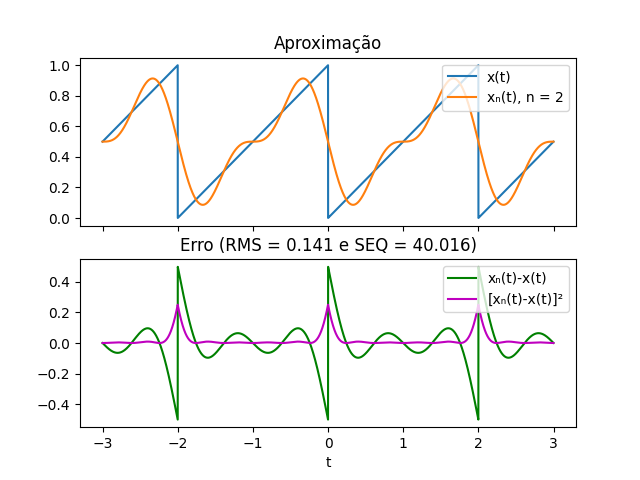
\includegraphics[width=0.9\linewidth]{dente_de_serra_n_2.png}
	\centering
	\caption{$n=2$.}
\end{figure}

\begin{figure}[h!]
	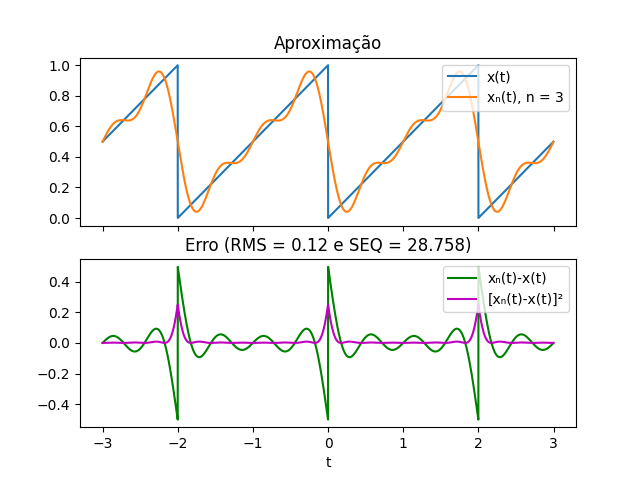
\includegraphics[width=0.9\linewidth]{dente_de_serra_n_3.png}
	\centering
	\caption{$n=3$.}
\end{figure}

\begin{figure}[h!]
	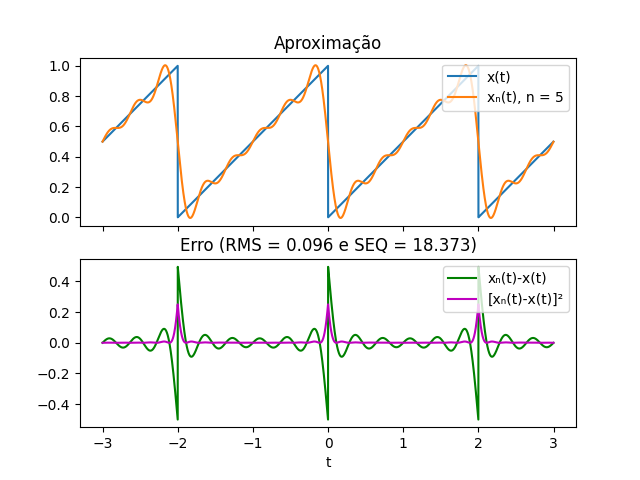
\includegraphics[width=0.9\linewidth]{dente_de_serra_n_5.png}
	\centering
	\caption{$n=5$.}
\end{figure}

\begin{figure}[h!]
	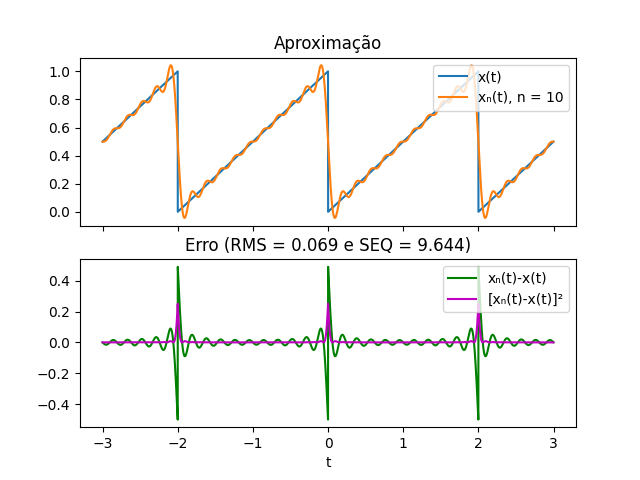
\includegraphics[width=0.9\linewidth]{dente_de_serra_n_10.png}
	\centering
	\caption{$n=10$.}
\end{figure}

\begin{figure}[h!]
	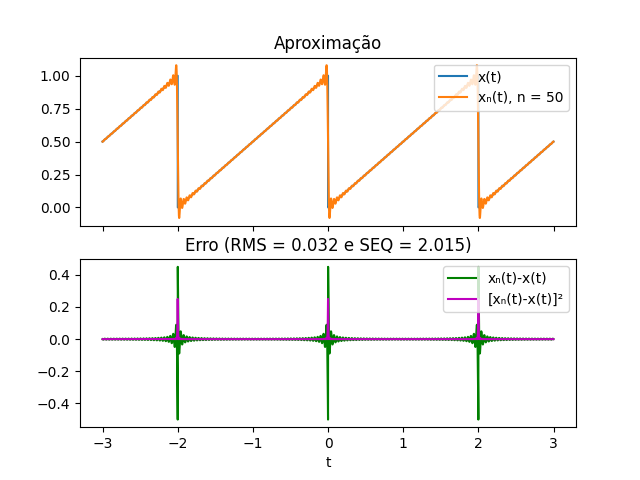
\includegraphics[width=0.9\linewidth]{dente_de_serra_n_50.png}
	\centering
	\caption{$n=50$.}
\end{figure}

\FloatBarrier
\pagebreak
Podemos fazer uma realizar uma simulação para vários valores de $n$ para verificar que, quanto mais termos da série nós somarmos, menor o erro se tornará em ambas as métricas:

\begin{figure}[h!]
	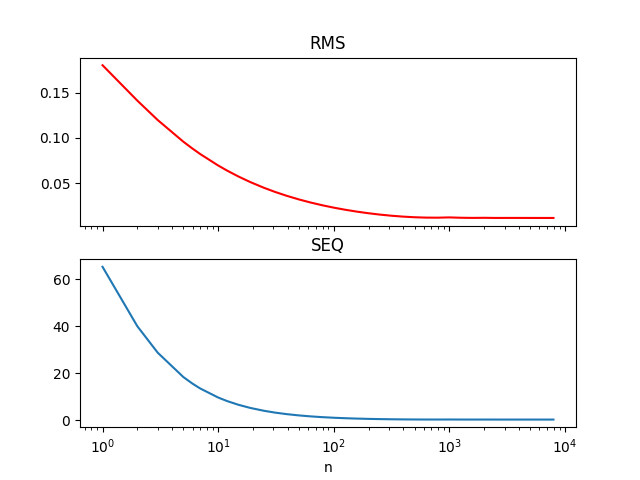
\includegraphics[width=0.9\linewidth]{dente_de_serra_erro.png}
	\centering
	\caption{Erros SEQ e RMS em função de $n$ para o sinal dente de serra.}
\end{figure}
\FloatBarrier

Com o aumento da quantidade de termos, a série aproxima o sinal original cada vez melhor, mas nos pontos de descontinuidade nós sempre temos picos que ultrapassam o sinal desejado. Este fenômeno é chamado de fenômeno de Gibbs.

\section{Avaliação por série de Fourier da onda quadrada}

\subsection{Análise teórica}

Temos um sinal periódico definido em um de seus períodos da seguinte forma:

\begin{equation*}
	x(t)=\begin{dcases}
		\;\;\,1&\text{se}\quad\quad\;\;\, 0<t\leq10\\
		-1&\text{se}\quad -10<t\leq0
	\end{dcases}
\end{equation*}

Seu período fundamental é $T_0=20$ e a sua frequência fundamental é $\omega_0=\frac{\pi}{10}$.

\subsubsection{Cálculo de $a_k$}

Vamos aplicar a seguinte fórmula:

\begin{equation*}
	a_k=\frac{1}{T_0}\int_{-\frac{T}{2}}^{\frac{T}{2}}x(t)\,e^{-\j k\omega_0t}dt=
	\frac{1}{20}\int_{-10}^{10}x(t)\,e^{-\frac{\j k\pi}{10}\,t}dt
\end{equation*}

Quebrando a integral em duas partes:

\begin{equation*}
	a_k=\frac{1}{20}\left(\int_{-10}^{0}x(t)\,e^{-\frac{\j k\pi}{10}\,t}dt+\int_{0}^{10}x(t)\,e^{-\frac{\j k\pi}{10}\,t}dt\right)
\end{equation*}

\begin{equation*}
	a_k=\frac{1}{20}\left(\int_{-10}^{0}-e^{-\frac{\j k\pi}{10}\,t}dt+\int_{0}^{10}e^{-\frac{\j k\pi}{10}\,t}dt\right)
\end{equation*}

\begin{equation*}
	a_k=\frac{1}{20}\left(\int_{0}^{10}e^{-\frac{\j k\pi}{10}\,t}dt-\int_{-10}^{0}e^{-\frac{\j k\pi}{10}\,t}dt\right)
\end{equation*}

\begin{equation*}
	a_k=\frac{1}{20}\left(\left[-\frac{10\,e^{-\frac{\j k\pi}{10}\,t}}{\j\pi k}\right]_{t=0}^{t=10}-\left[-\frac{10\,e^{-\frac{\j k\pi}{10}\,t}}{\j\pi k}\right]_{t=-10}^{t=0}\right)
\end{equation*}

\begin{equation*}
	a_k=\left[\frac{e^{-\frac{\j k\pi}{10}\,t}}{2\j\pi k}\right]_{t=10}^{t=0}+\left[\frac{e^{-\frac{\j k\pi}{10}\,t}}{2\j\pi k}\right]_{t=-10}^{t=0}
\end{equation*}

\begin{equation*}
	a_k=\frac{1}{2\j\pi k}-\frac{e^{-\j k\pi}}{2\j\pi k}+\frac{1}{2\j\pi k}-\frac{e^{\j k\pi}}{2\j\pi k}
\end{equation*}

\begin{equation*}
	a_k=\frac{1}{\j\pi k}-\frac{e^{-\j k\pi}}{2\j\pi k}-\frac{e^{\j k\pi}}{2\j\pi k}
\end{equation*}

\begin{equation*}
	a_k=\frac{1}{\j\pi k}-\frac{1}{\j\pi k}\left(\frac{e^{\j k\pi}+e^{-\j k\pi}}{2}\right)
\end{equation*}

\begin{equation*}
	a_k=\frac{1}{\j\pi k}-\frac{1}{\j\pi k}\cdot\cos(k\pi)
\end{equation*}

\begin{equation*}
	a_k=\frac{1-\cos(k\pi)}{\j k\pi}
\end{equation*}

\begin{equation*}
	a_k=\begin{dcases}
		\frac{2}{\j k\pi}&\text{para }k\text{ ímpar}\\
		\;\:\,0&\text{para }k\text{ par}
	\end{dcases}
\end{equation*}

\subsubsection{Série de Fourier}

A série exponencial completa vai ser a seguinte:

\begin{equation*}
	x(t)=\sum_{k=-\infty}^{\infty}a_k\,e^{\j k\omega_0t}
\end{equation*}

\begin{equation*}
	x(t)=\sum_{k=-\infty}^{\infty}\frac{1-\cos(k\pi)}{\j k\pi}\cdot e^{\frac{\j k\pi t}{10}}
\end{equation*}

\subsubsection{Série truncada de Fourier}

A série truncada vai ser a mesma coisa que a série normal, mas o somatório é finito, do índice $k=-n$ até $k=n$:

\begin{equation*}
	x_n(t)=\sum_{k=-n}^{n}a_k\,e^{\j k\omega_0t}
\end{equation*}

\begin{equation*}
	x_n(t)=\sum_{k=-n}^{n}\frac{1-\cos(k\pi)}{\j k\pi}\cdot e^{\frac{\j k\pi t}{10}}
\end{equation*}

\subsection{Simulação numérica}

Vamos utilizar as mesmas métricas de erro que utilizamos com o sinal dente de serra, mas desta vez vamos utilizar $\Delta t=10^{-2}$.

\FloatBarrier

\begin{figure}[h!]
	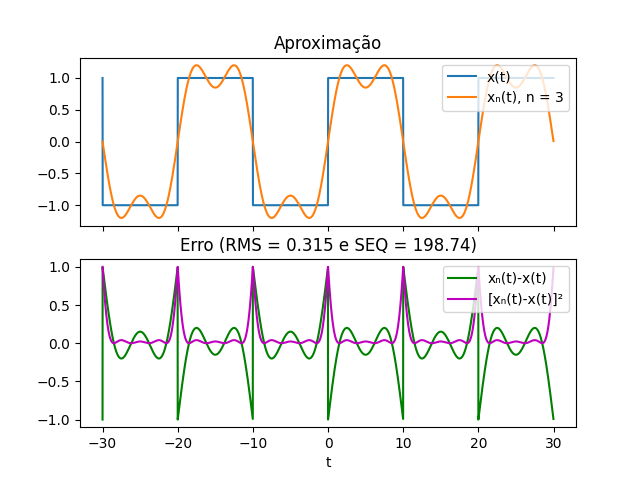
\includegraphics[width=0.9\linewidth]{onda_quadrada_n_3.png}
	\centering
	\caption{$n=3$.}
\end{figure}

\begin{figure}[h!]
	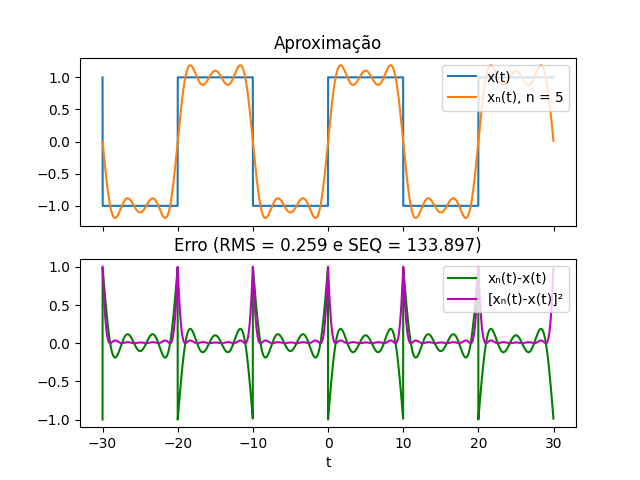
\includegraphics[width=0.9\linewidth]{onda_quadrada_n_5.png}
	\centering
	\caption{$n=5$.}
\end{figure}

\begin{figure}[h!]
	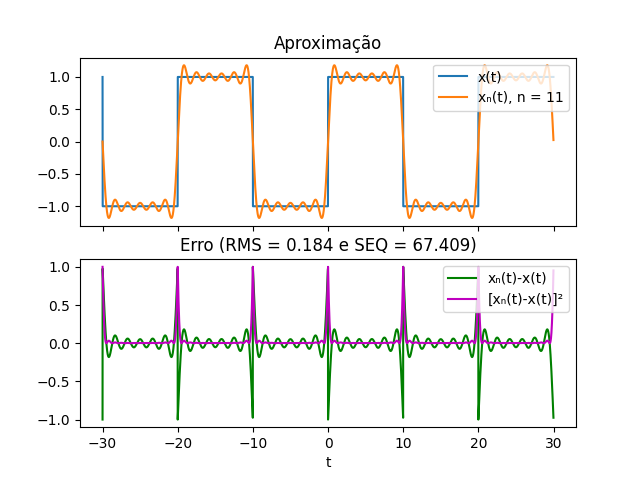
\includegraphics[width=0.9\linewidth]{onda_quadrada_n_11.png}
	\centering
	\caption{$n=11$.}
\end{figure}

\begin{figure}[h!]
	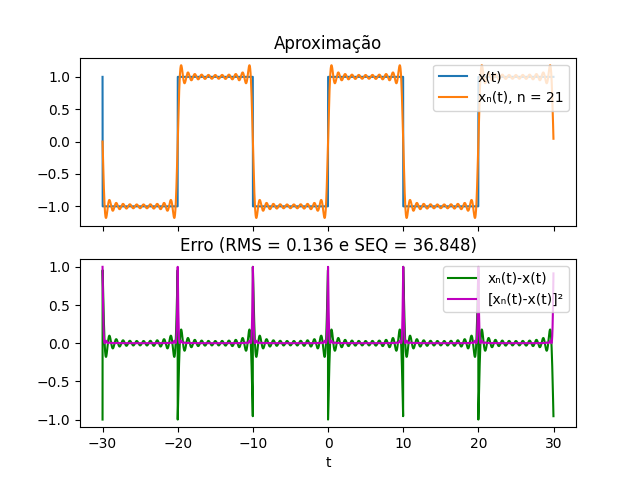
\includegraphics[width=0.9\linewidth]{onda_quadrada_n_21.png}
	\centering
	\caption{$n=21$}
\end{figure}

\begin{figure}[h!]
	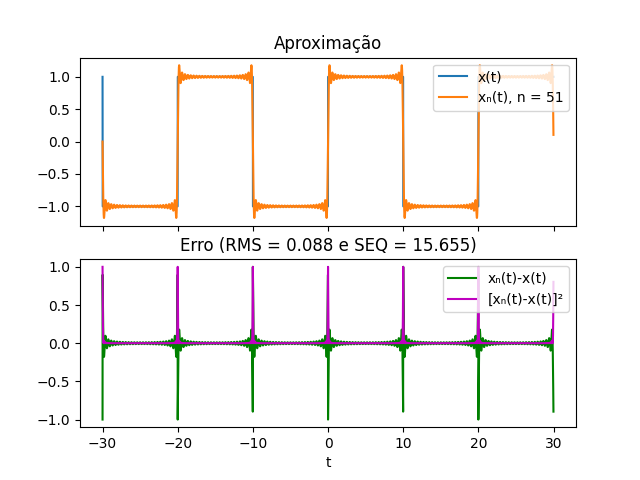
\includegraphics[width=0.9\linewidth]{onda_quadrada_n_51.png}
	\centering
	\caption{$n=51$.}
\end{figure}

\FloatBarrier

Mais uma vez, o erro diminui com o aumento da quantidade de termos da série, mas o fenômeno de Gibbs continua presente. Vamos dar uma olhada na onda quadrada no domínio da frequência:
\FloatBarrier
\begin{figure}[h!]
	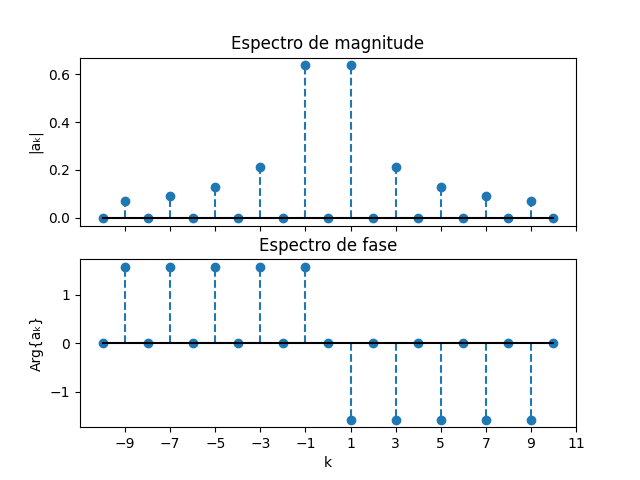
\includegraphics[width=0.9\linewidth]{onda_quadrada_freq.png}
	\centering
	\caption{Espectros de magnitude e fase da onda quadrada.}
\end{figure}
\FloatBarrier

\section{Filtragem da onda quadrada pelo circuito RC}

\subsection{Análise teórica}

\subsubsection{Cálculo de $H(\j\omega)$}

Vamos começar determinando a função de transferência do filtro, aplicando a transformada de Laplace na equação diferencial:

\begin{equation*}
	\tau\deriv{y}{t}{}+y(t)=x(t)
\end{equation*}

\begin{equation*}
	\lt{\tau\deriv{y}{t}{}+y(t)}=\lt{x(t)}
\end{equation*}

\begin{equation*}
	\tau sY(s)+Y(s)=X(s)
\end{equation*}

\begin{equation*}
	Y(s)\cdot(\tau s+1)=X(s)
\end{equation*}

\begin{equation*}
	H(s)=\frac{Y(s)}{X(s)}=\frac{1}{\tau s+1}
\end{equation*}

A resposta em frequência pode ser calculada a partir da função de transferência:

\begin{equation*}
	H(j\omega)=H(s)\biggr\rvert_{s=\j\omega}=\frac{1}{\j\omega\tau+1}
\end{equation*}

\subsubsection{Aplicação do filtro na onda quadrada}

A resposta em frequência multiplica cada uma das componentes de $x(t)$ de acordo com as suas frequências:

\begin{equation*}
	x(t)=\sum_{k=-\infty}^{\infty}a_k\,e^{\j k\omega_0t}
\end{equation*}

\begin{equation*}
	y(t)=\sum_{k=-\infty}^{\infty}H(\j k\omega_0)\,a_k\,e^{\j k\omega_0t}
\end{equation*}

\begin{equation*}
	y(t)=\sum_{k=-\infty}^{\infty}\frac{1}{\frac{\j k\pi\tau}{10}+1}\,\frac{1-\cos(k\pi)}{\j k\pi}\,e^{\frac{\j k\pi t}{10}}
\end{equation*}

\begin{equation*}
	y(t)=\sum_{k=-\infty}^{\infty}\frac{10}{\j k\pi\tau+10}\,\frac{1-\cos(k\pi)}{\j k\pi}\,e^{\frac{\j k\pi t}{10}}
\end{equation*}

\subsection{Simulação numérica}

Vamos plotar os gráficos de $x(t)$ e $y_n(t)$ para diferentes valores de $n$:

\FloatBarrier
\begin{figure}[h!]
	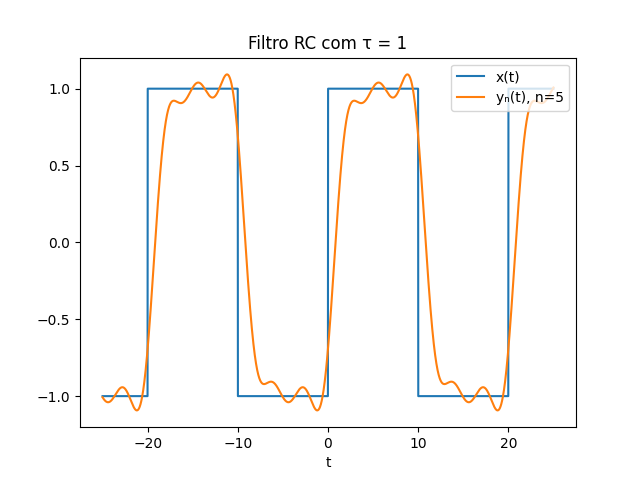
\includegraphics[width=0.9\linewidth]{filtro_n_5_t_1.png}
	\centering
	\caption{$n=5$.}
\end{figure}

\begin{figure}[h!]
	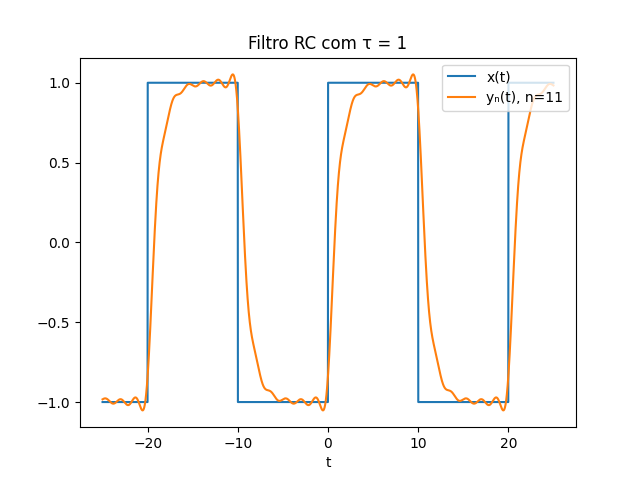
\includegraphics[width=0.9\linewidth]{filtro_n_11_t_1.png}
	\centering
	\caption{$n=11$.}
\end{figure}

\begin{figure}[h!]
	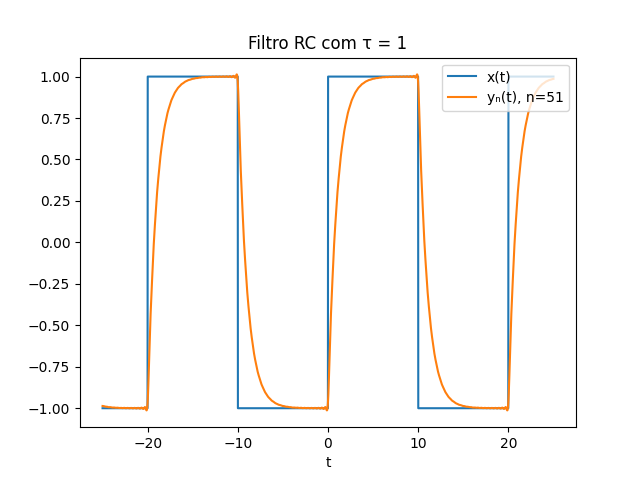
\includegraphics[width=0.9\linewidth]{filtro_n_51_t_1.png}
	\centering
	\caption{$n=51$.}
\end{figure}

\begin{figure}[h!]
	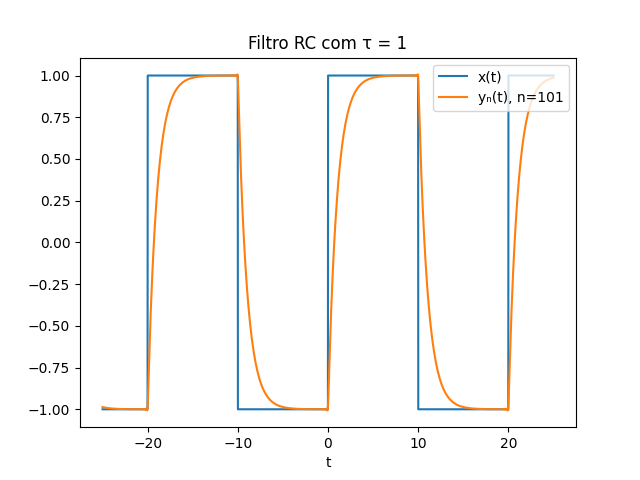
\includegraphics[width=0.9\linewidth]{filtro_n_101_t_1.png}
	\centering
	\caption{$n=101$.}
\end{figure}
\FloatBarrier

Conforme aumentamos a quantidade de termos da série, cada vez mais a curva se aproxima das exponenciais crescentes e decrescentes características de capacitores carregando e descarregando.

Vamos alterar o valor de $\tau$ e ver como o circuito reage:

\FloatBarrier
\begin{figure}[h!]
	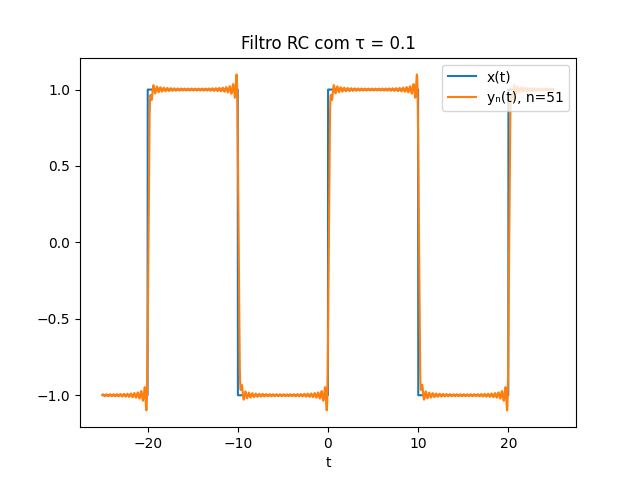
\includegraphics[width=0.9\linewidth]{filtro_n_51_t_0.1.png}
	\centering
	\caption{$\tau=\num{0.1}$.}
\end{figure}

\begin{figure}[h!]
	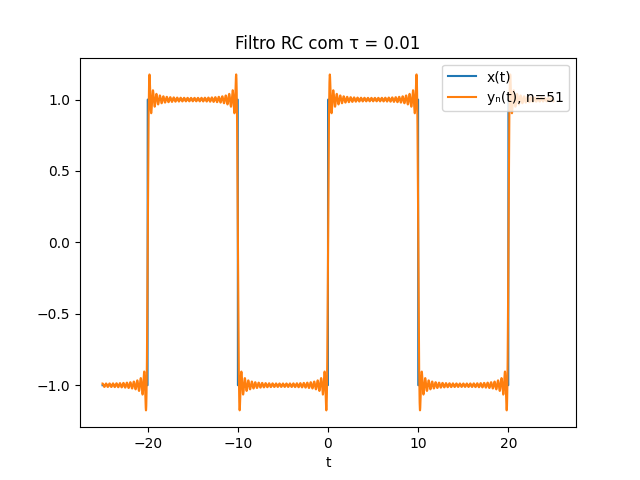
\includegraphics[width=0.9\linewidth]{filtro_n_51_t_0.01.png}
	\centering
	\caption{$\tau=\num{0.01}$.}
\end{figure}
\FloatBarrier

Como podemos ver, a diminuição da constante de tempo faz com que o capacitor carregue e descarregue de forma mais rápida, o que torna a sua tensão muito próxima da própria onda quadrada. Em outras palavras, a frequência de corte foi aumentada.

Vamos dar uma olhada no gráfico de $H(k\omega_0)$:

\FloatBarrier
\begin{figure}[h!]
	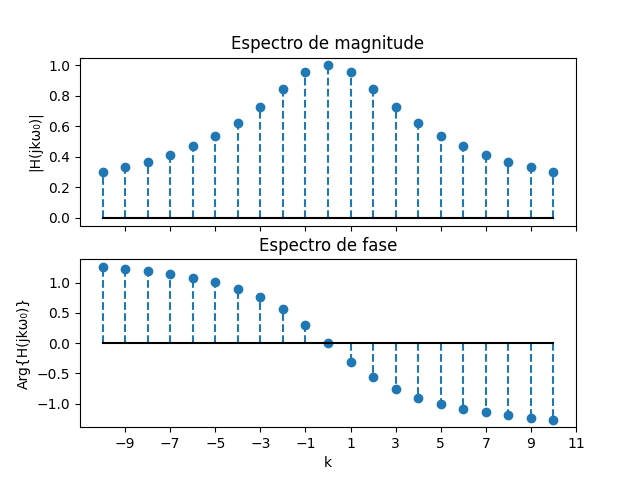
\includegraphics[width=0.9\linewidth]{H(kw0).png}
	\centering
	\caption{Gráfico de $H(\j k\omega_0)$.}
\end{figure}
\FloatBarrier

Como esperado, quanto maior a frequência, maior vai ser a atenuação aplicada pelo filtro. Como o capacitor apresenta inércia de tensão, ele resiste às mudanças muito rápidas, atenuando as frequências mais altas, característica de um filtro passa-baixa.

\end{document}
